\chapter{Desenvolvimento}
\section{Hardware}
\subsection{TIVA e seus pontos fracos}
O desenvolvimento foi iniciado com a placa EK-TM4C1294XL, que contém o controlador TM4C1294NCPDT. 
Embora a placa possua capacidade 
!! Placa EK-TM4C1294XL que contém o controlador TM4C1294NCPDT

!! Não possui firmware específico para essa aplicação (recepção e reprodução de áudio)

!! Não possui I2S

!! I2S pode ser emulado com dois I2C, porém apresenta dificuldades com outros componentes da placa

!! Software próprio se tornou instável a ponto de impedir o desenvolvimento

!! Precisaria de uma placa com componentes próprios (codec, DAC, Conector P2) para serem iniciados os testes
\subsection{STM32F769I-DISCO e suas vantagens}

!! Já possui firmware base para comunicação USB

!! Possui saída de áudio e display LCD com touch; facilita protótipos

!! Possui I2S, sendo possível seu uso nativo

!! Controlador STM32F769NI possui capacidade um pouco maior de processamento 


\subsection{Possíveis hosts para o device}

Diversos sistemas operacionais possuem as especificações necessárias para se comunicarem com o dispositivo sem necessidade de instalação de drivers. Os sistemas mais utilizados em computadores pessoais atualmente, como Windows, Linux e MacOS, possuem drivers para comunicação com dispositivos de áudio por USB.

Além disso, sistemas operacionais de dispositivos móveis também possuem compatibilidade direta com o dispotivivo. Nessa lista, incluem-se os dois sistemas mais utilizados, Android e iOS.

Embora os computadores ou dispositivos móveis nos quais os sitemas operacionais estão inseridos possivelmente já possuam uma solução de saída de áudio, é possível ser feita a sobreposição desse sistema, onde o áudio é enviado ao dispositivo ao invés de pela saída padrão.

\begin{figure}[!h]
  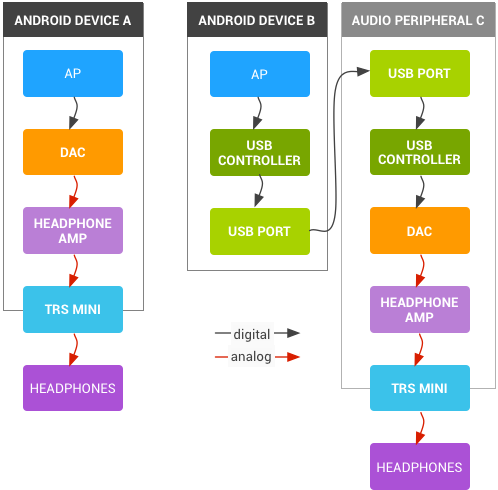
\includegraphics[scale=0.5]{figuras/usb-android-dscs.png}
  \caption{!! TROCAR POR VERSÃO DE AUTORIA PRÓPRIA !!}
  \label{fig:synchronousMode}
\end{figure}


\subsection{Componentes}

!! Serial Audio Interface Codec
% https://www.st.com/resource/en/product_training/STM32F7_Peripheral_SAI.pdf

\color{red}
An audio codec with four DACs and two ADCs is connected to the SAI interface of the
STM32F769NIH6. It communicates with the STM32F769NIH6 via an I2C bus shared with
the touch panel of the LCD DSI:
• The analog line input is connected to the ADC of the codec device via an audio jack
(CN6).
• The analog line output is connected to the DAC of the codec device via an audio jack
(CN7).
• Two external speakers can be connected to the codec device via the JP2 for the left
speaker and JP3 for the right speaker.
• Four digital microphones (ST MEMS microphone) are available on the
32F769IDISCOVERY Discovery board. They are connected to the input digital
microphones of the STM32F769NIH6 and the DFSDM functionality manages them.
• One coaxial connector (CN12) is implemented on the 32F769IDISCOVERY to receive
external audio data compatible with SPDIF specifications.
• One coaxial connector (CN8) is implemented on the 32F769IDISCOVERY to output
external audio data compatible with SPDIF specifications.

For audio playback, the STM32 board is recognized by the PC (USB Host) as a USB
speaker. The PC sends audio samples to the board via the USB. The STM32 MCU
configures the audio codec via the I2C
\color{black}

!! DAC

!! Output jack

\section{Firmware}
\subsection{HAL, BSP e CMSIS}
Este projeto conta com a utilização de camadas de abstração de hardware que ???. Entre elas, estão a HAL (Hardware Abstraction Layer), BSP (Board Support Package) e CMSIS (Common Microcontroller Software Interface Standard).
\\[10pt]
% https://en.wikipedia.org/wiki/Hardware_abstraction
% https://www.techopedia.com/definition/4288/hardware-abstraction-layer-hal
% https://emteria.com/learn/hardware-abstraction-layer


A \textit{Hardware Abstraction Layer (HAL)} é uma camada de bibliotecas de código que possui a função de entregar uma interface de desenvolvimento padronizada que permita interações com o hardware sem necessidade do conhecimento direto do hardware em questão 
% [[FONTE]](https://emteria.com/learn/hardware-abstraction-layer).

Isso permite uma maior portabilidade do código, o qual se torna compatível com qualquer hardware que também esteja incluso nessa camada de abstração.
Uma HAL é comumente acessível como uma API que realiza o trabalho de inicialização, configuração e acesso a um hardware específico. Para este projeto, foi utilizada a HAL V1.2.6, lançada em 29 de junho de 2018.
\\[10pt]

A \textit{Board Support Package (BSP)} é uma coleção de APIs, drivers e arquivos de configuração que tem como intuito facilitar o desenvolvimento em uma placa específica. 
Para este projeto, foi utilizado a BSP da placa STM32F769I-DISCO.
\\[10pt]

O \textit{Common Microcontroller Software Interface Standard (CMSIS)} é um conjunto de ferramentas, \textit{frameworks} e funcionalidades que implementam funcionalidades, mecânicas e utilidades comumente utilizadas no desenvolvimento embarcado, com o intuito de reduzir o atrito inicial do desenvolvimento, evitar re-trabalhos e reduzir e o tempo até o mercado de um produto até o mercado. Ele funciona em paralelo à Hardware Abstraction Layer, inclusive dependendo da versão específica dessa abstração para alguma de suas funcionalidades.

!! As partes não são diretamente compatíveis: BSP, HAL e CMSIS devem estar em versões corretas para que sua interação ocorra corretamente

!! A versão de BSP com a base para a comunicação de áudio USB utilizada uma versão antiga da HAL

!! As bibliotecas de interface humana (\textit{display}, \textit{touch}, serial) utilizavam uma versão mais atualizada da HAL

!! A ideia inicial era de portar o código antigo da BSP de áudio USB para a nova HAL

!! As mudanças entre versões da HAL são bem abrangentes, incluindo parâmetros de funções e estruturas de dados

!! Atualizar a versão antiga da BSP precisaria quase de uma reescrita do código de conexão com a HAL

!! Foi preferido realizar o processo inverso, e realizar um \textit{downgrade} da HAL das funcionalidades de interface humana para serem compatíveis com o código BSP de áudio USB

!! O principal impasse desse processo foi devido a \textit{hard faults} que ocorriam quando os códigos eram inicializados simultaneamente. Cada módulo funcionava corretamente em isolamento, porém causavam a placa a parar de responder caso fossem inicializados juntos

!! Foi identificado que um problema de timing ocorria entre as bibliotecas, onde alguns registradores eram acessados ou escritos em momentos que estavam sendo acessados por outra biblioteca. A adição de um atraso entre as inicializações das diferentes funcionalidades deixou a inicialização da placa um pouco mais lenta, porém resolveu completamente o problema de \textit{hard faults} no momento de inicialização

% [https://www.arm.com/technologies/cmsis#:~:text=Common Microcontroller Software Interface Standard,to market for new devices](https://www.arm.com/technologies/cmsis#:~:text=Common%20Microcontroller%20Software%20Interface%20Standard,to%20market%20for%20new%20devices).

% https://deepbluembedded.com/stm32-hal-library-tutorial-examples/

% https://www.st.com/resource/en/product_training/STM32G0-Ecosystem-STM32Cube-G0-Firmware-Package.pdf

% https://arm-software.github.io/CMSIS_5/General/html/index.html

\subsection{Configuração como dispositivo de áudio USB}
Algumas configurações precisam ser enviadas na conexão com a fonte para que o dispositivo seja reconhecido corretamente como um dispositivo de áudio. Duas das principais configurações necessárias são os VIDs e PIDs, ambos números de 16 bits tipicamente representados em hexadecimal.

\subsection{Seleção de parâmetros para transmissão}

!! Explicar por que foi escolhido 48k (comentar das poucas diferenças em taxas maiores de amostragem e até problemas de fold back/fold over

!! Comentar do uso de 2 canais (stereo)

!! Comentar do uso de 16 bit (mostrar relação com noise floor já aceitável)

!! Comentar de buffer size ser 10240 bytes (com margem de 1 packet)

% // computes the nominal size(number of bytes) of an audio packet required for one millisecond
% // e.g. for 48KHZ   / 24 bits / stereo, the required size is 48 * 3 * 2
% //      for 44.1KHZ / 16 bits / stereo, the required size is 44 * 2 * 2
% #define AUDIO_MS_PACKET_SIZE(freq,channel_count,res_byte) (((uint32_t)((freq) /1000)) * (channel_count) * (res_byte)) 

% // computes the maximum size(number of bytes) of an audio packet required for one millisecond(without computing the sample added for synchronization)
% // e.g. for 48KHZ   / 24 bits / stereo, required size is 48 * 3 * 2
% //      for 44.1KHZ / 16 bits  /stereo, required size is 45 * 2 * 2
% #define AUDIO_MS_MAX_PACKET_SIZE(freq,channel_count,res_byte) AUDIO_MS_PACKET_SIZE(freq+999,channel_count,res_byte)

!! Packet para 1ms em 48KHz e 16 bits stereo contém 48 * (16 / 8) * 2 = 192bytes

% https://en.wikipedia.org/wiki/USB_Implementers_Forum

\textit{VIDs (Vendor IDs)} são números que identificam um fabricante ou fornecedor de dispositivos USB. Esse identificador é fornecido pelo USB Implementers Forum, necessitando de licenças anuais de custo elevado. Algumas fabricantes de microcontroladores permitem o uso de sua licença para fins não comerciais ou de pequena escala. Este projeto utiliza o vendor ID da STMicroelectronics (0x0483)

\textit{PIDs (Product IDs)} são números que identificam o dispositivo de maneira diferente para o sistema operacional ao qual ele está se conectando. Esse identificador varia de acordo com cada fornecedor.

Para esse dispositivo ser reconhecido como uma saída de áudio da STMicroelectronics, ele precisa informar ao sistema operacional que está se conectando o identificador 0x5730.

\subsection{Armazenamento (buffer circular)}
Como o modo de tranferência não possui correção de erro nem bufferização de dados, precisamos utilizar de um armazenamento temporário para podermos manipular e enviar o dado para frente.
\begin{figure}[!h]
  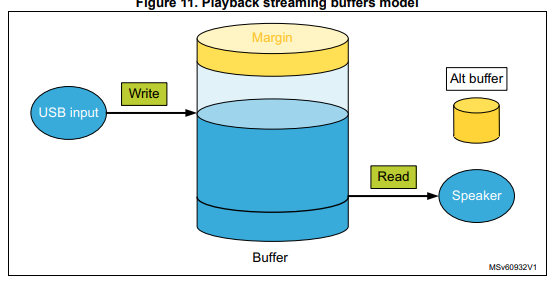
\includegraphics[scale=0.5]{figuras/circular-buffer.png}
  \caption{!! TROCAR POR VERSÃO DE AUTORIA PRÓPRIA !!}
  \label{fig:circularBuffer}
\end{figure}

Para se adequar ao padrão produtor-consumidor utilizado na transmissão USB, um buffer circular é utilizado. 

Ponteiros de leitura e escrita são utilizados para indicação de onde novos pacotes devem ser lidos e onde devem ser escritos, respectivamente. O ponteiro de leitura é administrado pelo nó de saída de áudio, e o de escrita pelo nó de entrada USB.

!!Explicar como dados são inseridos no buffer!!. O ponteiro de escrita é então incrementado para refletir a presença dos novos dados presentes no buffer.

!! Explicar como dados são consumidos do buffer!!. O ponteiro de leitura é incrementado para refletir esta leitura.

Através de DMA, os dados são então transferidos para o SAI (e em sequência para o codec).

Para todas as escritas e leituras serem de uma área contínua de memória, uma margem é adicionada ao *buffer*. Isso permite que dados sejam escritos de maneira contínua, mesmo caso o ponteiro de escrita esteja próximo do fim do buffer.

Caso dados sejam escritos de forma que ultrapassem o fim do buffer, a quantidade restante é escrita na margem. Posteriormente, esses dados são corretamente re-escritos no começo do buffer. 

Em casos que não existem dados suficientes para serem escritos ao SAI, um buffer alternativo contendo apenas zeros é utilizado.


\subsection{Processamento de sinal (interceptador)}
Para possibilitar a alteração dos dados recebidos antes que eles sejam transmitidos ao nó de saída, um interceptador foi criado e adicionado como passo intermediário.

O interceptador é um conjunto de métodos que tem como objetivo receber o posicionamento dos dados originais no \textit{buffer}, e transformá-los de acordo com o filtro especificado. Essa transformação é feita antes que o ponteiro de leitura atinja essa parte do \textit{buffer}.

São enviadas informações de posição inicial dos dados, tamanho do pacote, e ponteiros de função para os filtros que devem ser aplicados a cada canal (direito e esquerdo)

Os dados são então iterados em \textit{frames} que possuem informação de dois samples (referentes aos dois canais stereo).

\begin{minted}{c}
    void AudioUserDsp_FrameToSamples(
    uint8_t* framePointer, 
    int16_t* leftSamplePointer, 
    int16_t* rightSamplePointer
    )
    {
      *leftSamplePointer  = framePointer[1] * 256 + framePointer[0];
      *rightSamplePointer = framePointer[3] * 256 + framePointer[2];
    }
\end{minted}

Cada um dos samples dos canais são então armazenados em variáveis temporárias. 

Cada filtro provido é então aplicado ao sample específico a seu canal, modificando-o. 

Finalmente, os samples são convertidos novamente em um único frame, e o valor final desse frame é atribuído à posição original do frame provido no \textit{buffer}.

\begin{minted}{c}
    void AudioUserDsp_SamplesToFrame(
    uint8_t* framePointer, 
    int16_t* leftSamplePointer, 
    int16_t* rightSamplePointer
    )
    {
      framePointer[0] = ((uint16_t)*leftSamplePointer) % 256;
      framePointer[1] = ((uint16_t)*leftSamplePointer) / 256;
      framePointer[2] = ((uint16_t)*rightSamplePointer) % 256;
      framePointer[3] = ((uint16_t)*rightSamplePointer) / 256;
    }
\end{minted}


\subsection{IHM (LCD + Touch)}
A interface homem-máquina é feita com a utilização do LCD embarcado na placa de desenvolvimento. Através dela, o usuário pode verificar a situação atual do sistema, incluindo quais filtros estão ativos no momento.

!! SCREENSHOT 1 !!

O dispositivo também conta com resposta à toque, permitindo com que o usuário interaja diretamente com os dados mostrados em tela. Um sistema de botões radiais foi desenvolvido para permitir que o usuário possa alternar entre os filtros em tempo real.

!! Foi feita uma configuração de botões extensível, para que a interface com o usuário possa ser posteriormente personalizada. Os botões podem ser ligados entre si, para que apenas um fique ativo por vez, ou serem independentes. Os botões podem ser posicionados em qualquer posição vertical e horizontal da tela, e sua cor quando desligados e ligados pode ser personalizada.
A adição de novos botões pode ser feita com pouco acréscimo de código, apenas estendendo a lista de botões já criados.

\section{PDS}

\color{red}
IIR filters are generally implemented in two-pole sections called biquads because
they are described with a biquadratic equation in the z-domain. Higher order filters
are designed using cascaded biquad sections, i.e., a 6-pole filter requires 3 biquad
sections.

The general digital filter equation is shown in Figure 6.32 which gives rise to the
general transfer function H(z) which contains polynomials in both the numerator
and the denominator. The roots of the denominator determine the pole locations of
the filter, and the roots of the numerator determine the zero locations. Although it
is possible to construct a high order IIR filter directly from this equation (called the
direct form implementation), accumulation errors due to quantization errors (finite
wordlength arithmetic) may give rise to instability and large errors. For this reason,
it is common to cascade several biquad sections with appropriate coefficients rather
than use the direct form implementation. The biquads can be scaled separately and
then cascaded in order to minimize the coefficient quantization and the recursive
accumulation errors. Cascaded biquads execute more slowly than their direct form
counterparts, but are more stable and minimize the effects of errors due to finite
arithmetic errors.
\color{black}

!! Implementado filtro inicial passa baixa para validação de funcionamento
\begin{sourcecode}[!ht]
\centering
\begin{minted}{c}
    int16_t AudioUserDsp_LowPassFilter(
    int16_t sample, 
    uint32_t iteration
    )
    {
      a0 = 0.011050373933114971f;
      a1 = 0.022100747866229942f;
      a2 = 0.011050373933114971f;
      b1 = -1.3368583644305965f;
      b2 = 0.3810598601630564f;
    
      double fInSample = (float)(sample >> 2);
      double fOutSample = 
          a0 * fInSample 
        + a1 * in_z1 
        + a2 * in_z2
        - b1 * out_z1
        - b2 * out_z2;
    
    
      in_z2   = in_z1;
      in_z1   = fInSample;
      out_z2  = out_z1;
      out_z1  = fOutSample;
    
    
      return (int16_t)fOutSample;
    }

\end{minted}
\caption{Código de filtro passa baixa empregado pelo interceptador}\label{code:CML}
\end{sourcecode}
!! Combinação de filtros IIR Biquadráticos é a melhor solução para a implementação de filtros passa faixa

!! Os pontos de queda de -3db entre filtros adjacentes devem ser iguais, para que não haja influencia de um passa faixa no filtro próximo
% https://electronics.stackexchange.com/questions/104330/poor-mans-equalizer-with-a-few-digital-bandpass-filters-how-to-overlap-band-e

\begin{sourcecode}[htb]
\caption{\label{codigo:classeFoo}Classe Aluno}
\begin{lstlisting}[frame=single, language=c]
    int16_t AudioUserDsp_LowPassFilter(
    int16_t sample, 
    uint32_t iteration
    )
    {
      a0 = 0.011050373933114971f;
      a1 = 0.022100747866229942f;
      a2 = 0.011050373933114971f;
      b1 = -1.3368583644305965f;
      b2 = 0.3810598601630564f;
    
      double fInSample = (float)(sample >> 2);
      double fOutSample = 
          a0 * fInSample 
        + a1 * in_z1 
        + a2 * in_z2
        - b1 * out_z1
        - b2 * out_z2;
    
    
      in_z2   = in_z1;
      in_z1   = fInSample;
      out_z2  = out_z1;
      out_z1  = fOutSample;
    
    
      return (int16_t)fOutSample;
    }
\end{lstlisting}
\fonte{}
\end{sourcecode}